\chapter{Results}

\section{Maxwellian}

These are parameters for the calculation in Fig.~\ref{f:compareMaxwellian}.
Angle is $60^\circ$. 
Radar frequency is \SI{230}{\mega\hertz} which corresponds to EISCAT VHF and EISCAT 3D radars.  % Citation here?
Magnetic field strength is $10^{-5}$ \si{\tesla}.
The neutral, ion, and electron temperature are all $T_i=T_e=T_n=\SI{1000}{\kelvin}$.
The neutral number density is \SI{1.8e14}{\meter^{-3}}.
The plasma is quasineutral with $n_i=n_e=10^9$ \si{\meter^{-3}}.
Atomic oxygen is the ion species.
The numerical calculation is done using $n_{\max}$ of 2000 for the ions and 50 for the electrons (these two are expected to be overkill for the calculation).

\begin{figure}[!htb]
	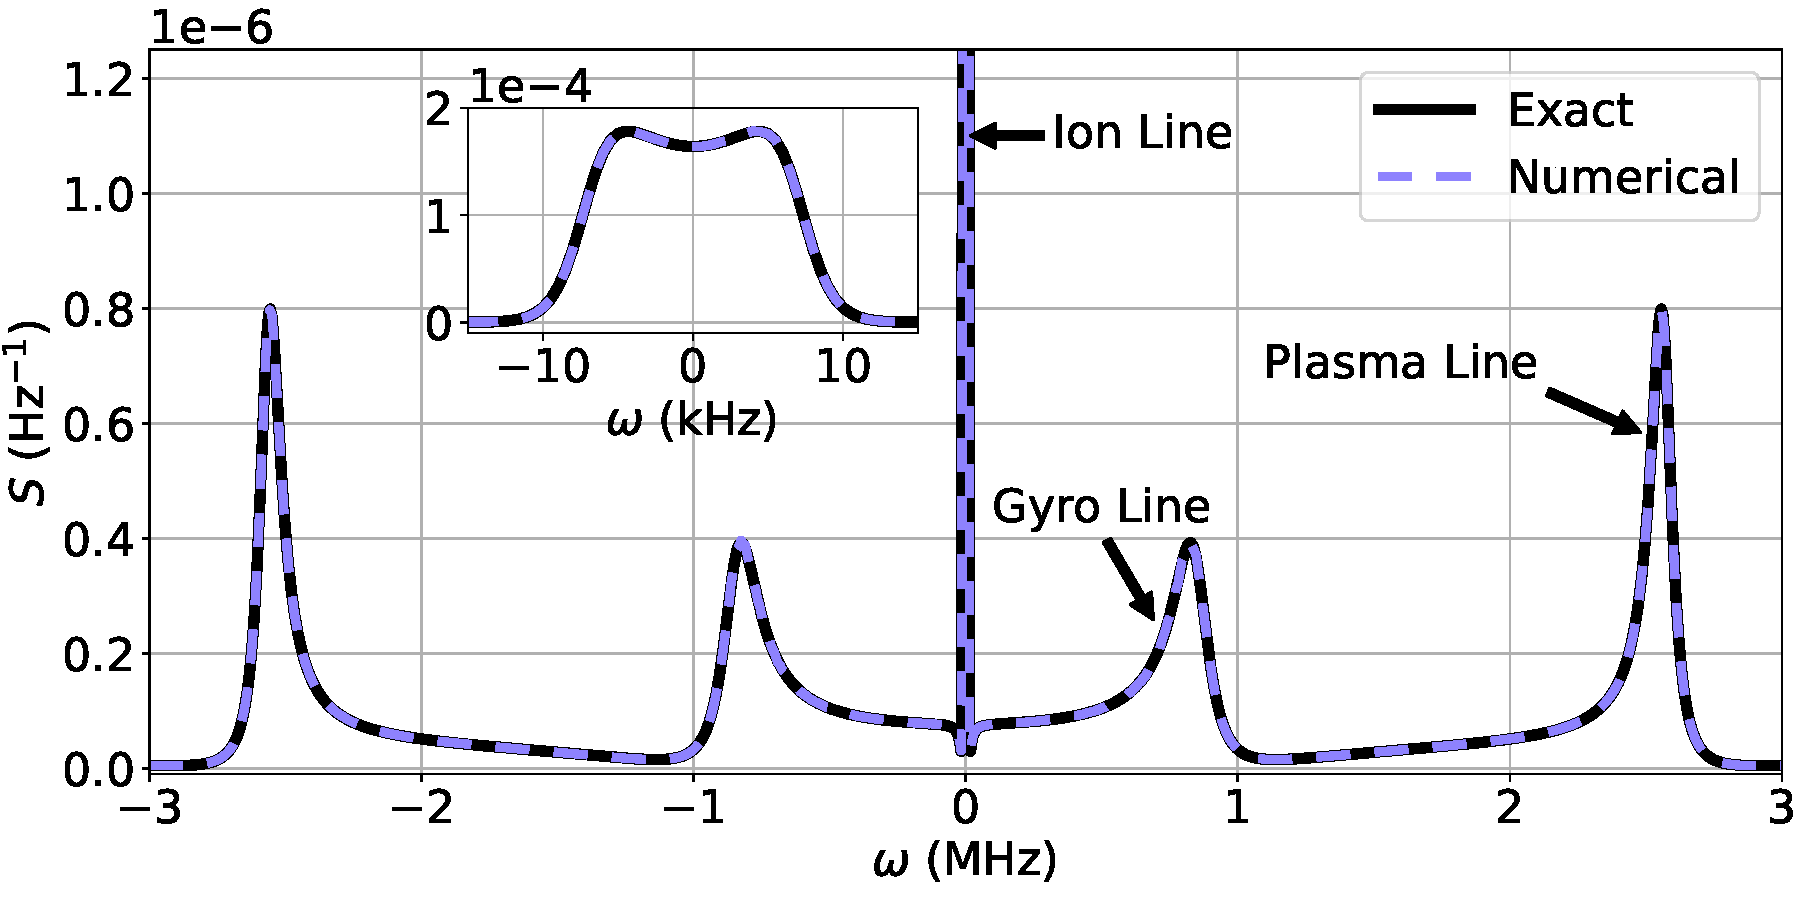
\includegraphics[width=\linewidth]{compareMaxwellian.pdf}
	\caption{Comparison between exact solution and numerical solution for a Maxwellian plasma.}
	\label{f:compareMaxwellian}
\end{figure}


\section{Toroidal}

\begin{equation}
	f_0 = \frac{
		\exp\bigg( - \frac{2 D^* v_\perp}{v_{th,\perp}} \bigg) I_0 \bigg(  \frac{2 D^* v_\perp}{v_{th,\perp}} \bigg)  
		\exp \bigg(  -\frac{v_\parallel^2}{v_{th,\parallel}^2} - \Big[ \frac{v_\perp}{v_{th,\perp} } - D^* \Big]^2  \bigg)}{
		\pi^{3/2} v_{th,\parallel} v_{th,\perp}^{2}}
	\label{eq:toroidal_dist}
\end{equation}

These plots were made using Eq.~\ref{eq:toroidal_dist} as the base distribution with the exact parameters from \cite{goodwin2018} for the background plasma and radar parameters.
The equivalent temperature Maxwellian is calculated using the method in Sec.~\ref{s:equiv-temp-known}.

\begin{figure}[!htb]
	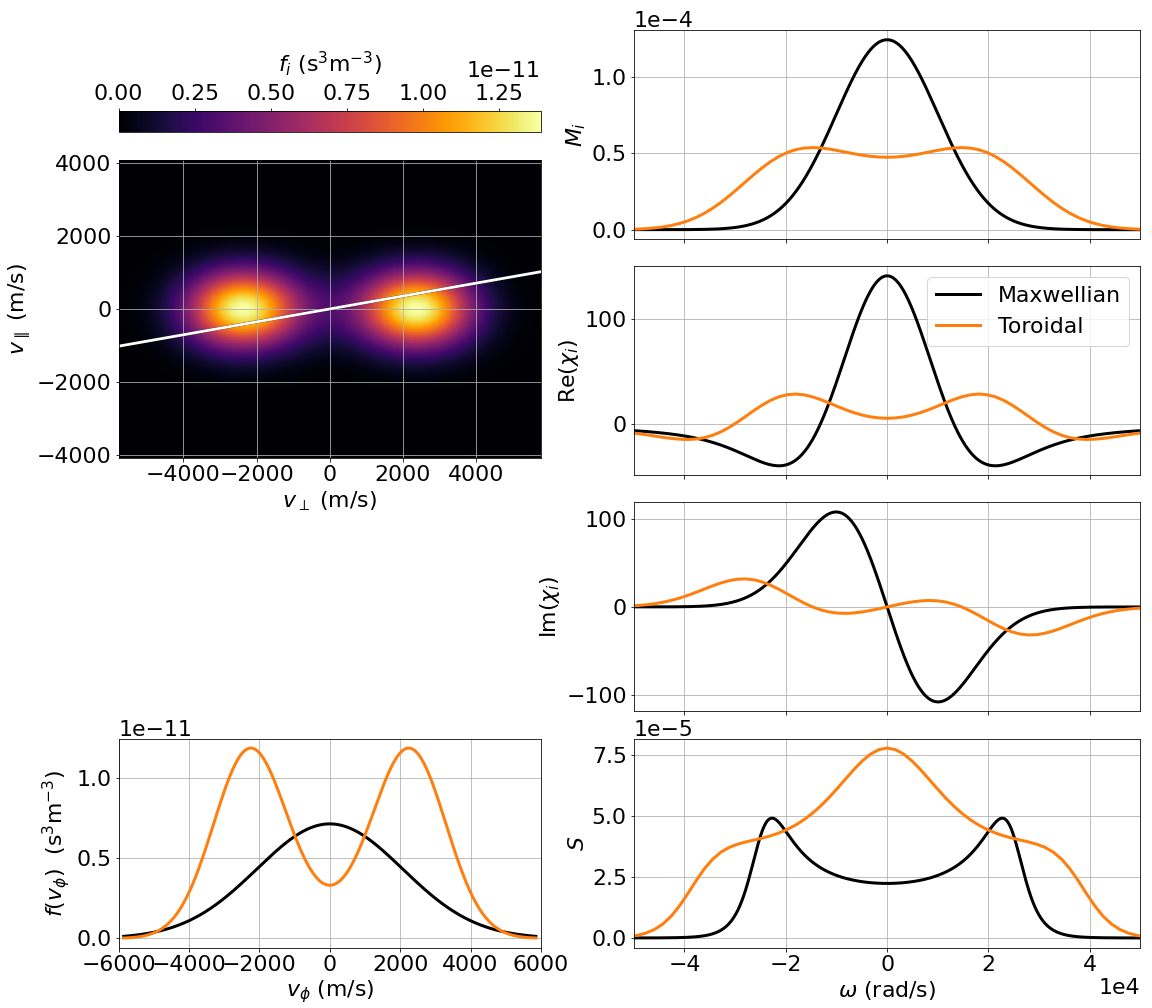
\includegraphics[width=\linewidth]{par2.3_perp2_Goodwin_Te4000_theta80_spectrum.png}
	\caption{Plots of plasma with toroidal ion distribution (orange line) compared to the equivalent temperature Maxwellian (black line).
	Color plot is the 2D $v_\perp v_\parallel$ representation of the distribution function from Eq.~\ref{eq:toroidal_dist}.
	The line on the color plot is the radar wave vector direction.
	The bottom left panel is the distribution function along wavevector direction.
	The top right panel is the modified distribution function.
	The middle right panels are the real and imaginary parts of the ion susceptibility, respectively.
	The bottom right panel is the ISR spectrum.
	The triple hump is shown, as expected based on \cite{goodwin2018}.}
	\label{f:toroidal}
\end{figure}


\section{Kappa}

These are results for a kappa distribution. See the \verb*|kappa_dist.nb| These have the form from \citep{livadiotis2015} as
\begin{equation}
	f_\kappa(\mathbf{v}) \sim \Bigg[   
	1 + \frac{1}{\kappa-d/2} \frac{\mathbf{v}^2}{v_{th}^2}
	\Bigg]^{-\kappa-1},
	\label{eq:kappa_base}
\end{equation}
where $\kappa$ is a constant that determines how long the tail of the distribution is (lower number means more high energy particles),
$v_{th}=\sqrt{2k_BT/m}$ is the thermal velocity,
and $d$ is the number of degrees of freedom (for our case, $d=3$).

In cylindrical coordinates, the square of the velocity becomes $\mathbf{v}^2=v_\perp^2+v_\parallel^2$. 
The normalization factor is found by taking the reciprocal of zeroth moment of Eq.~\ref{eq:kappa_base}.
Thus, the total disitribution function with three degrees of freedom is
\begin{equation}
	f_{\kappa}(v_\perp,v_\parallel) = 
	\frac{1}{\pi^{\frac{3}{2}} v_{th}^3 \big(\kappa-\frac{3}{2}\big)^{\frac{5}{2}}}
	\frac{\Gamma\big(\kappa+1\big)}{\Gamma\big(\kappa-\frac{3}{2}\big)}
	\Bigg( 1 + \frac{1}{\kappa-\frac{3}{2}} \frac{v_\perp^2+v_\parallel^2}{v_{th}^2}
	\Bigg)^{-\kappa-1},
	\label{eq:kappa_dist}
\end{equation}
where $\Gamma$ is the Gamma function.
Thus, based on the denominator Gamma term in this formulation, we can see that $kappa>3/2$ because the Gamma function is defined only for $z>0$.
As $\kappa\rightarrow\infty$, Eq.~\ref{eq:kappa_dist} tends to the Maxwellian distribution.
Furthermore, the temperature of this formulation of the kappa distribution is the same as that of the Maxwellian. 
In other words, the second moment is related to the thermal velocity in the same manner as in Maxwellian:
\begin{equation}
	\int_{-\infty}^\infty f_{\kappa}(v_\perp,v_\parallel) (v_\perp^2+v_\parallel^2) v_\perp dv_\perp dv_\parallel d\phi = 
	\frac{3}{2} v_{th}.
\end{equation}

% Throw some example plots of the kappa distribution here









